%
% File emnlp2020.tex
%
%% Based on the style files for ACL 2020, which were
%% Based on the style files for ACL 2018, NAACL 2018/19, which were
%% Based on the style files for ACL-2015, with some improvements
%%  taken from the NAACL-2016 style
%% Based on the style files for ACL-2014, which were, in turn,
%% based on ACL-2013, ACL-2012, ACL-2011, ACL-2010, ACL-IJCNLP-2009,
%% EACL-2009, IJCNLP-2008...
%% Based on the style files for EACL 2006 by 
%%e.agirre@ehu.es or Sergi.Balari@uab.es
%% and that of ACL 08 by Joakim Nivre and Noah Smith

\documentclass[11pt,a4paper]{article}
\usepackage[hyperref]{emnlp2020}
\usepackage{times}
\usepackage{latexsym}
\renewcommand{\UrlFont}{\ttfamily\small}

% This is not strictly necessary, and may be commented out,
% but it will improve the layout of the manuscript,
% and will typically save some space.
\usepackage{microtype}

\aclfinalcopy % Uncomment this line for the final submission
%\def\aclpaperid{***} %  Enter the acl Paper ID here

%\setlength\titlebox{5cm}
% You can expand the titlebox if you need extra space
% to show all the authors. Please do not make the titlebox
% smaller than 5cm (the original size); we will check this
% in the camera-ready version and ask you to change it back.


% Personal additions
\usepackage{amsmath}
\usepackage{float}
\usepackage[noabbrev,capitalize,nameinlink]{cleveref}
\usepackage{graphicx}
\usepackage{listings}

\newcommand\BibTeX{B\textsc{ib}\TeX}

\title{English Accent Classification with CNN-BiLSTM}

\author{Siwei Wang \\ \texttt{siweiw@umich.edu}}

\date{\today}

\begin{document}
\maketitle
\begin{abstract}
  In this paper, I test the hypothesis that a CNN can improve the ability of a BiLSTM to automatically classify accents in spoken English. The accent classes I used were Arabic, Dutch, English, French, Korean, Mandarin, Portuguese, Russian, and Spanish. The data was taken from the \href{https://accent.gmu.edu/}{Speech Accent Archive}. I discuss the preprocessing steps, and then describe the architecture of both the CNN and BiLSTM components of my model. Extra attention is given to how the two components are connected to one another. Next, I go over the results, in which I find that the CNN failed to improve BiLSTM performance. Finally, I bring up some ethical considerations and conclude with key takeaways and possible directions for future investigation.
\end{abstract}

\section{Introduction} \label{sec:introduction}

English has more second language speakers than the next five most popular second languages combined. It comes as no surprise that there are hundreds of accents to spoken English. In this paper, I tackle the problem of automatically classifying English accents. Several previous works have approached the accent classification task through both classical ML and deep learning. The latter methods have demonstrated some success in training a classifier, particularly with recurrent networks.

In this paper, I test the hypothesis that a specialized CNN may learn a useful representation of audio data that will improve the performance of RNN's. The organization of this paper is as follows. First, I conduct a brief survey of previous attempts at accent classification. Next, I describe the dataset. The heart of the paper will be in presenting the preprocessing and CNN-BiLSTM architecture. Finally, I discuss results as well as some ethical implications of such a system.

\section{Related Work} \label{sec:related_work}

There are several existing papers that have tried various architectures for the task of English accent classification. I present each previous work alongside its score \(S\), defined to be the product of test accuracy and number of accent labels, which indicates how many times more accurate the model is compared to random guessing.

\citet{chen} used SVM to get \(S = 1.19\). \citet{ahmed} introduced a CNN architecture they termed a ``variable filter net'' to achieve \(S = 2.11\). \citet{shih} implemented an LSTM to get \(S = 2.09\) test accuracy. \citet{sheng} reached \(S = 2.64\) with a CNN.

In most of the accent classifiers, audio data was first preprocessed using MFCC's. Note that using a CNN on mel spectrograms seemed to yield solid results as in \citet{ahmed} and \citet{sheng}. However, audio is inherently sequential, which lends itself to a recurrent model as in \citet{shih}. The success in both approaches leads to the possibility of applying a CNN and running the output through an LSTM in a way that preserves temporal structure.

\section{The Dataset} \label{sec:dataset}

All train, validation, and test data in this paper are derived from the \href{https://accent.gmu.edu/}{Speech Accent Archive}. Each recording consists of an individual reciting the following transcript.
\begin{quote}
  Please call Stella. Ask her to bring these things with her from the store: Six spoons of fresh snow peas, five thick slabs of blue cheese, and maybe a snack for her brother Bob. We also need a small plastic snake and a big toy frog for the kids. She can scoop these things into three red bags, and we will go meet her Wednesday at the train station.
\end{quote}

I downloaded the dataset from \href{https://www.kaggle.com/rtatman/speech-accent-archive}{Kaggle} and chose the 9 most common accents, which were Arabic, Dutch, English, French, Korean, Mandarin, Portuguese, Russian, and Spanish. The relative frequency of these recordings is displayed in \cref{fig:accent_freq}
\begin{figure}[h]
  \centering
  \caption{Frequency of Accents in Dataset}
  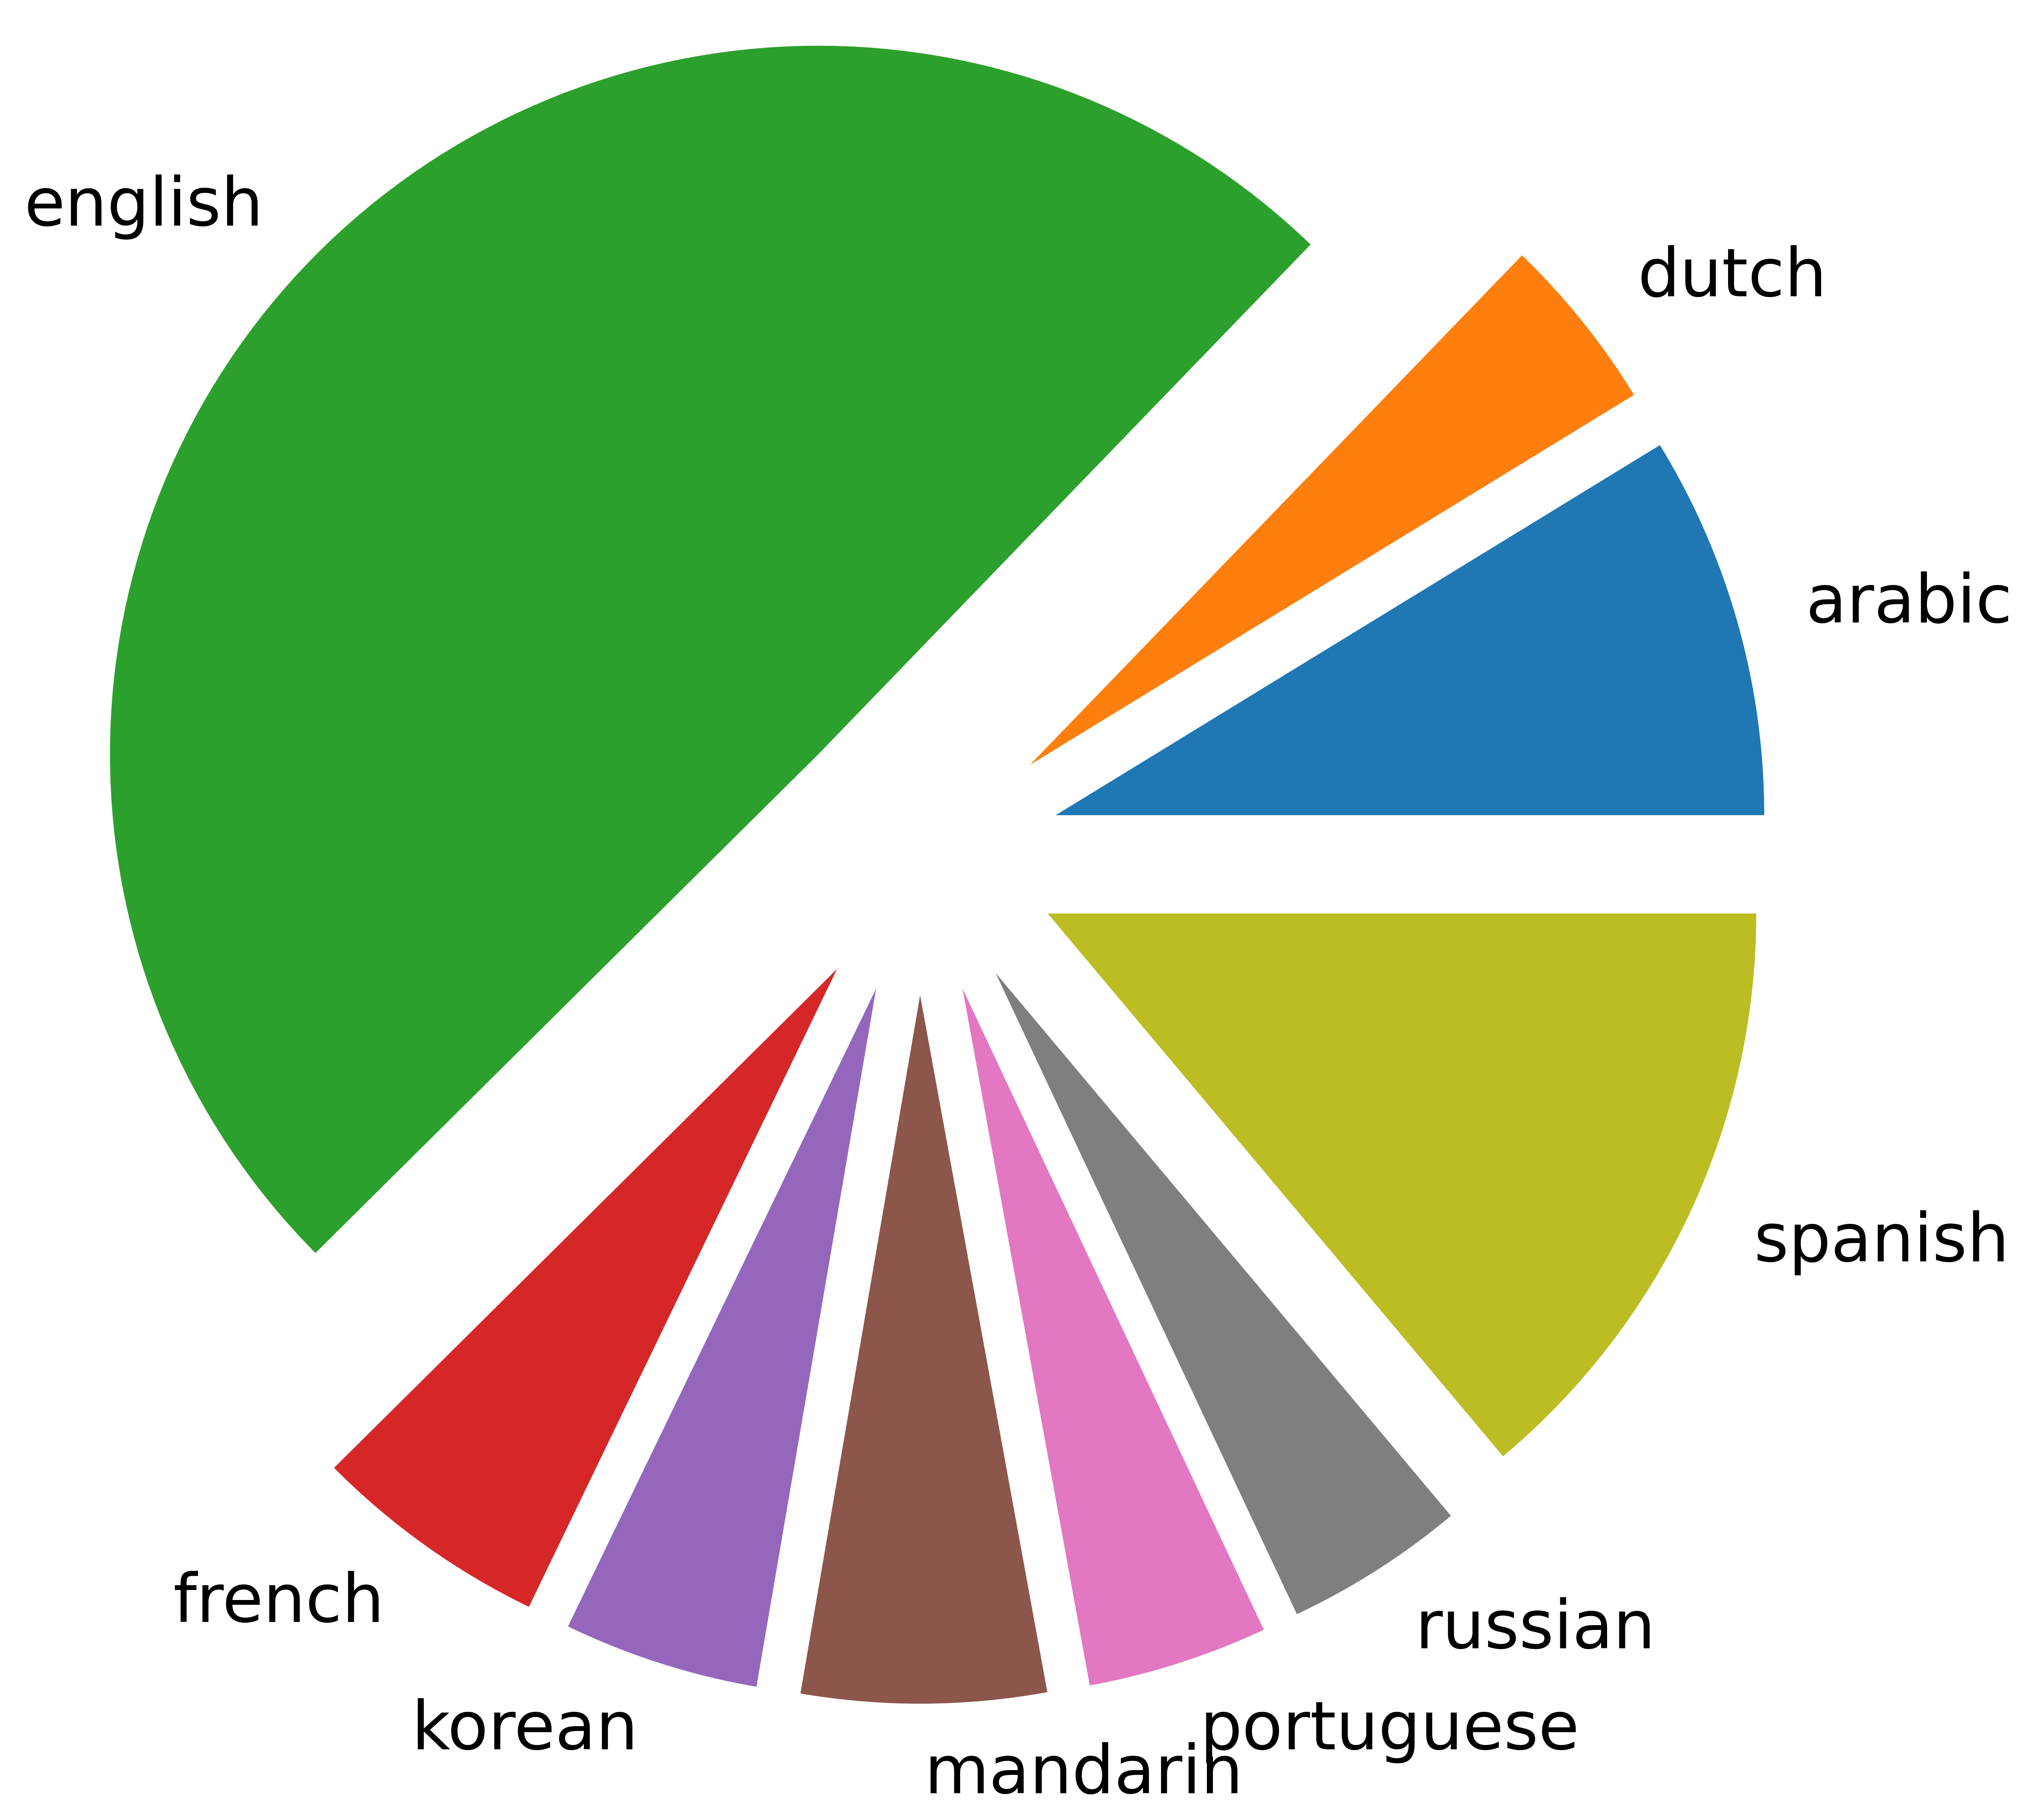
\includegraphics[width=.48\textwidth]{freq.png}
  \label{fig:accent_freq}
\end{figure}

There is a clear imbalance in the class labels, which I alleviate by assigning class weights to the labels during training. Each recording was downsampled to a uniform 8 kHz. I then plotted a histogram of the Euclidean norms of small audio snippets to get \cref{fig:norms}.
\begin{figure}[h]
  \centering
  \caption{Histogram of Norms from Audio Snippets}
  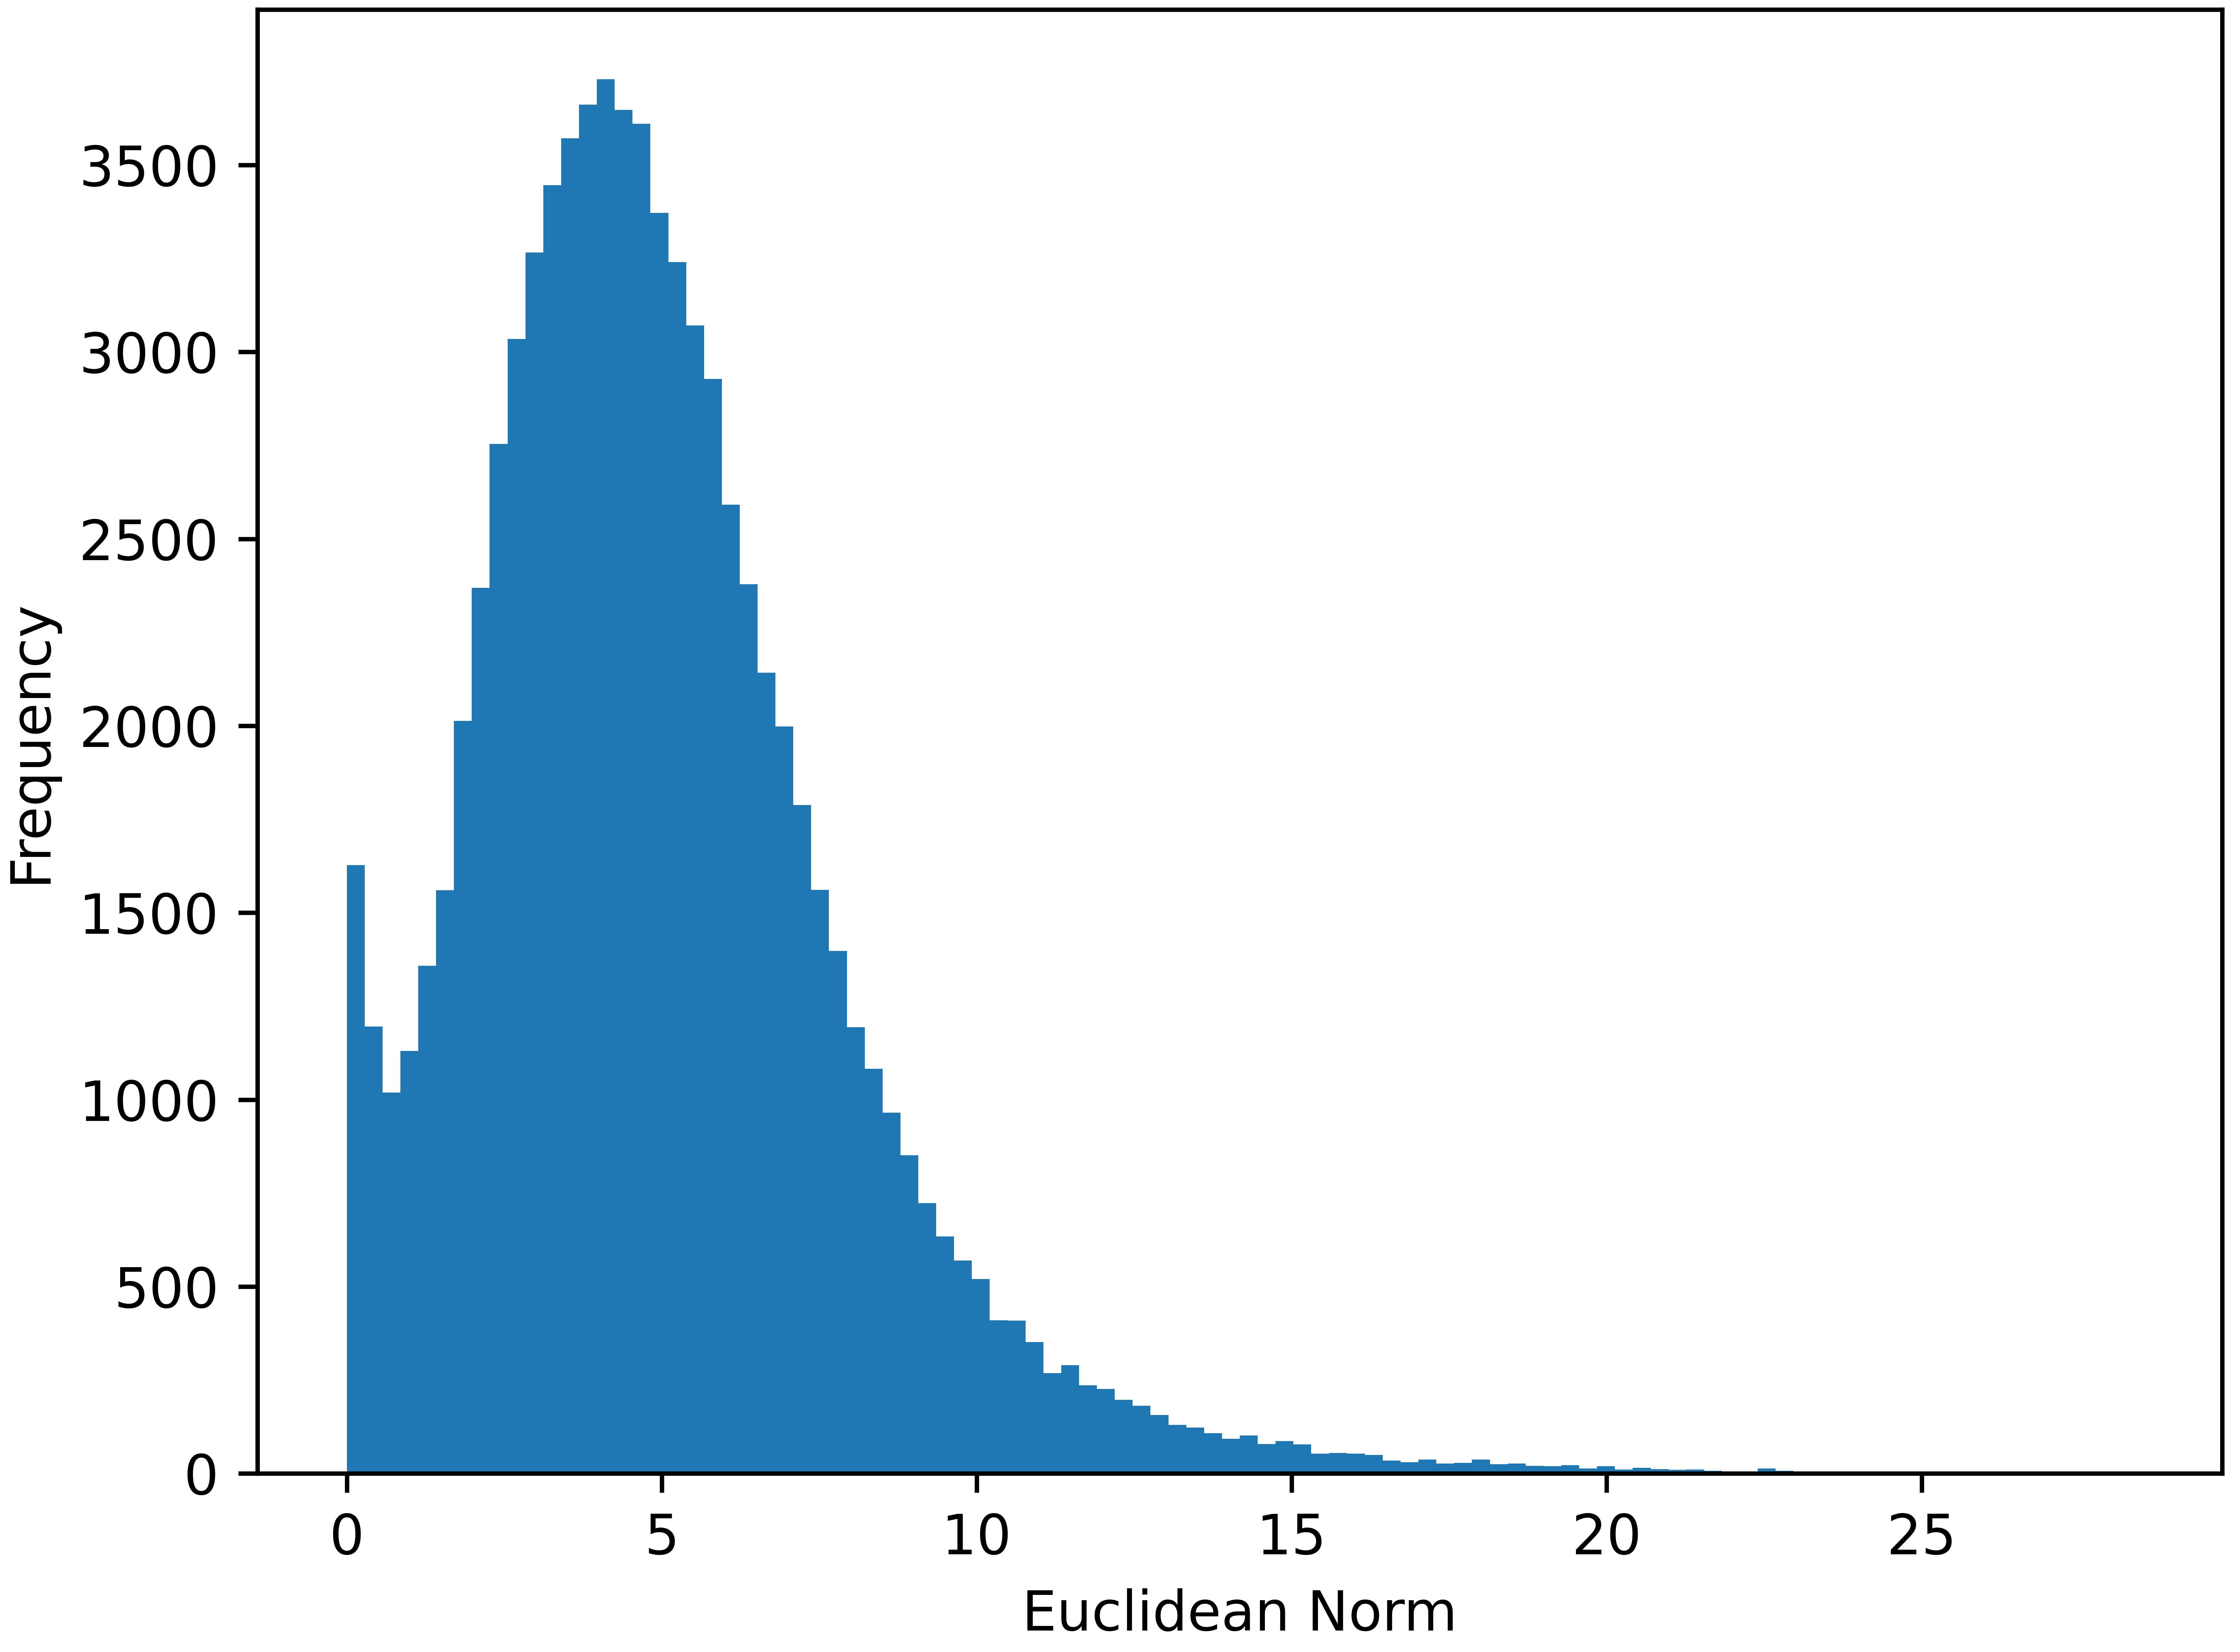
\includegraphics[width=.48\textwidth]{norms.png}
  \label{fig:norms}
\end{figure}

As expected, the distribution is approximately normal except for the spike near 0. This was caused by periods of relative silence, which I removed. The resulting histogram no longer has this spike. In addition, this step reduces background noise. These downsampled, silence-removed, mono-channel wav files are the starting point for later preprocessing steps.

In order to avoid correlation between the training and evaluation sets, I split the files into train, validation, and test sets (with ratio 0.8, 0.1, and 0.1 respectively) before preprocessing. The split was stratified to preserve relative label frequency.

\section{Preprocessing} \label{sec:preprocessing}

Each wav file is first decoded into a 1-D signal, represented as a vector \(A\) with components lying in the interval \([-1, 1]\). I then passed a sliding window with length \(25,000\) and step size \(5,000\) over the signal, creating a series of smaller 1-D frames, each of length \(25,000\). Define a mask \(M_i^j\) to be a vector of length equal to \(A\) such that
\begin{equation}
  M_i^j[t] = \begin{cases}
    1 & \text{if } i \leq t \leq j \\
    0 & \text{otherwise}
  \end{cases}
\end{equation}
Then the \(k^{th}\) frame of \(A\) is given by
\begin{equation}
  A \odot M_{5000k}^{5000k + 25000}
\end{equation}
where \(\odot\) denotes component-wise product.

For each frame, I produce a spectrogram, apply a mel filter bank with 128 filters, rescale to decibels, and standardize to mean 0 and standard deviation 1. The frequency range for the MFB was 0 kHz to 4 kHz. The result os these operations is a 2-D image with dimensions \(98 \times 128\) where 98 is the number of time steps. \cref{fig:mel_spec} shows a heatmap for a randomly chosen spectrogram.
\begin{figure}[h]
  \centering
  \caption{Mel Spectrogram of Audio Frame}
  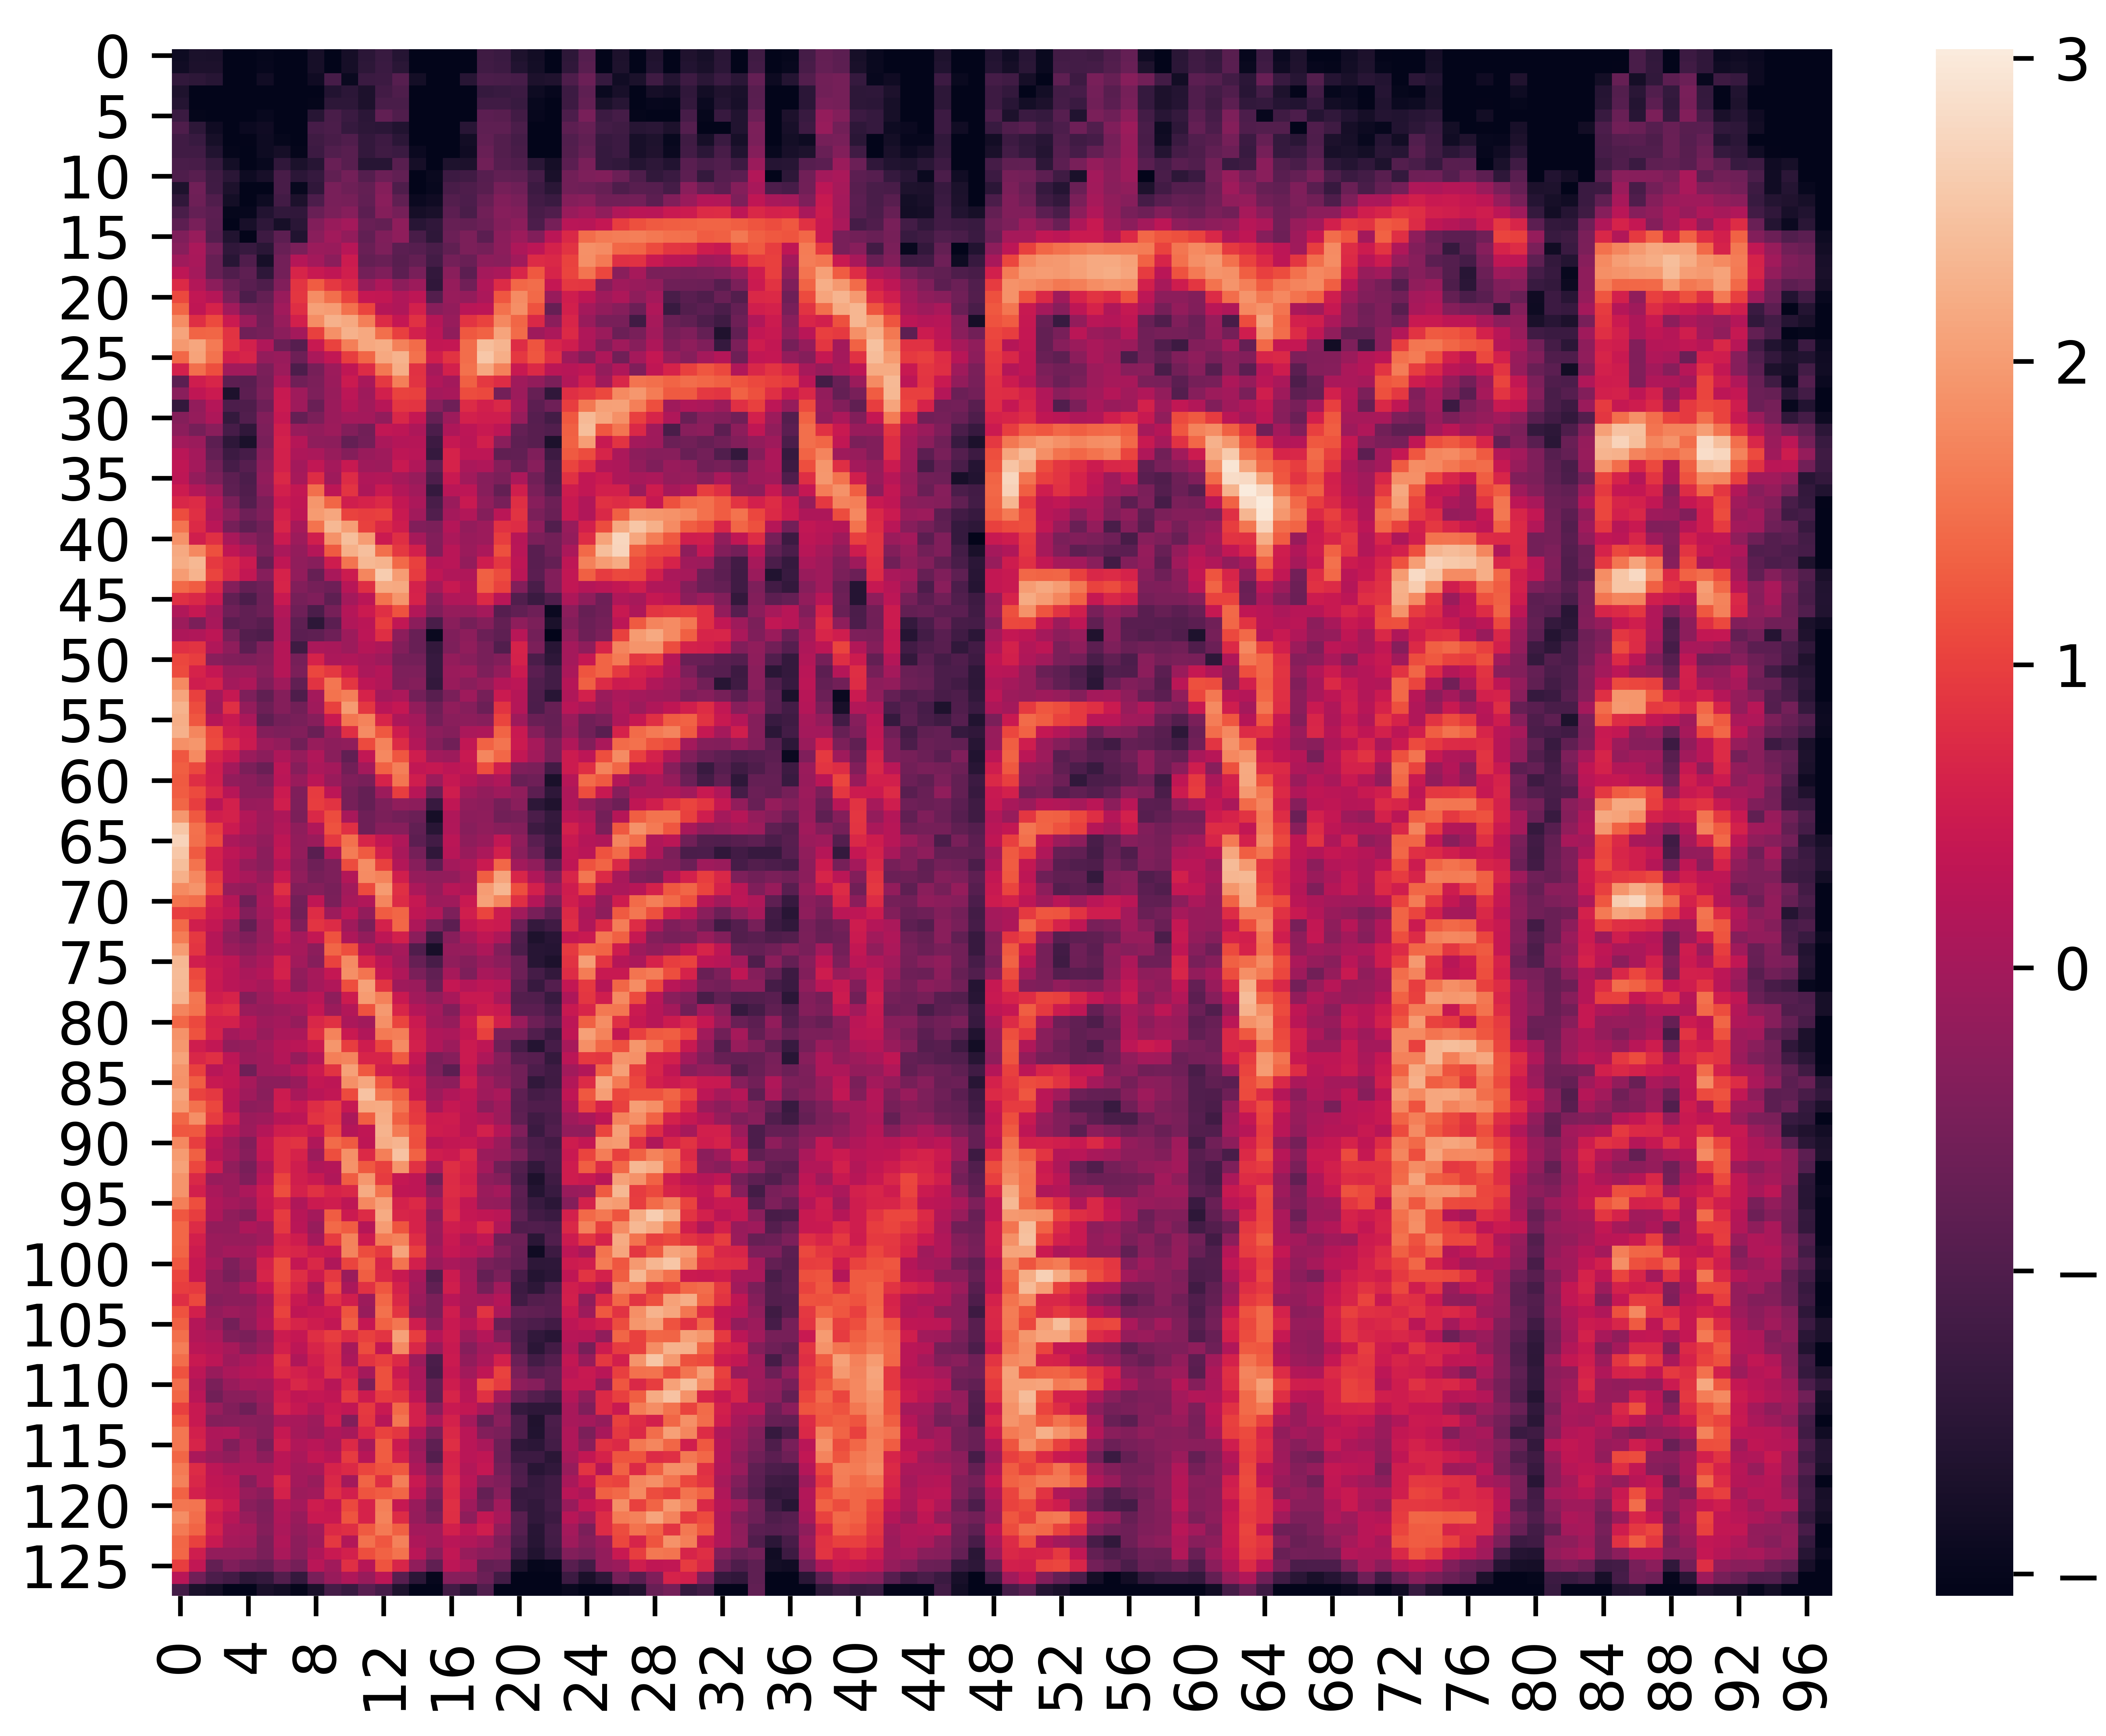
\includegraphics[width=.48\textwidth]{spec.png}
  \label{fig:mel_spec}
\end{figure}

Using fixed-length frames as opposed to the entire audio signal means that every input has the same number of time-steps. This simplifies the batching and training process and prevents recording length from a being a factor.

\section{The BiLSTM} \label{sec:bilstm}

A LSTM (short for long short term memory) is a specialized RNN capable of learning long-term dependencies. In \cref{fig:lstm_chain}, \(x_t\) is the input and \(h_t\) is the model's respective output at time step \(t\). In this case, \(x_t\) is comprised of 128 mel coefficients.
\begin{figure}[h]
  \centering
  \caption{LSTM Chain \citep{olah}}
  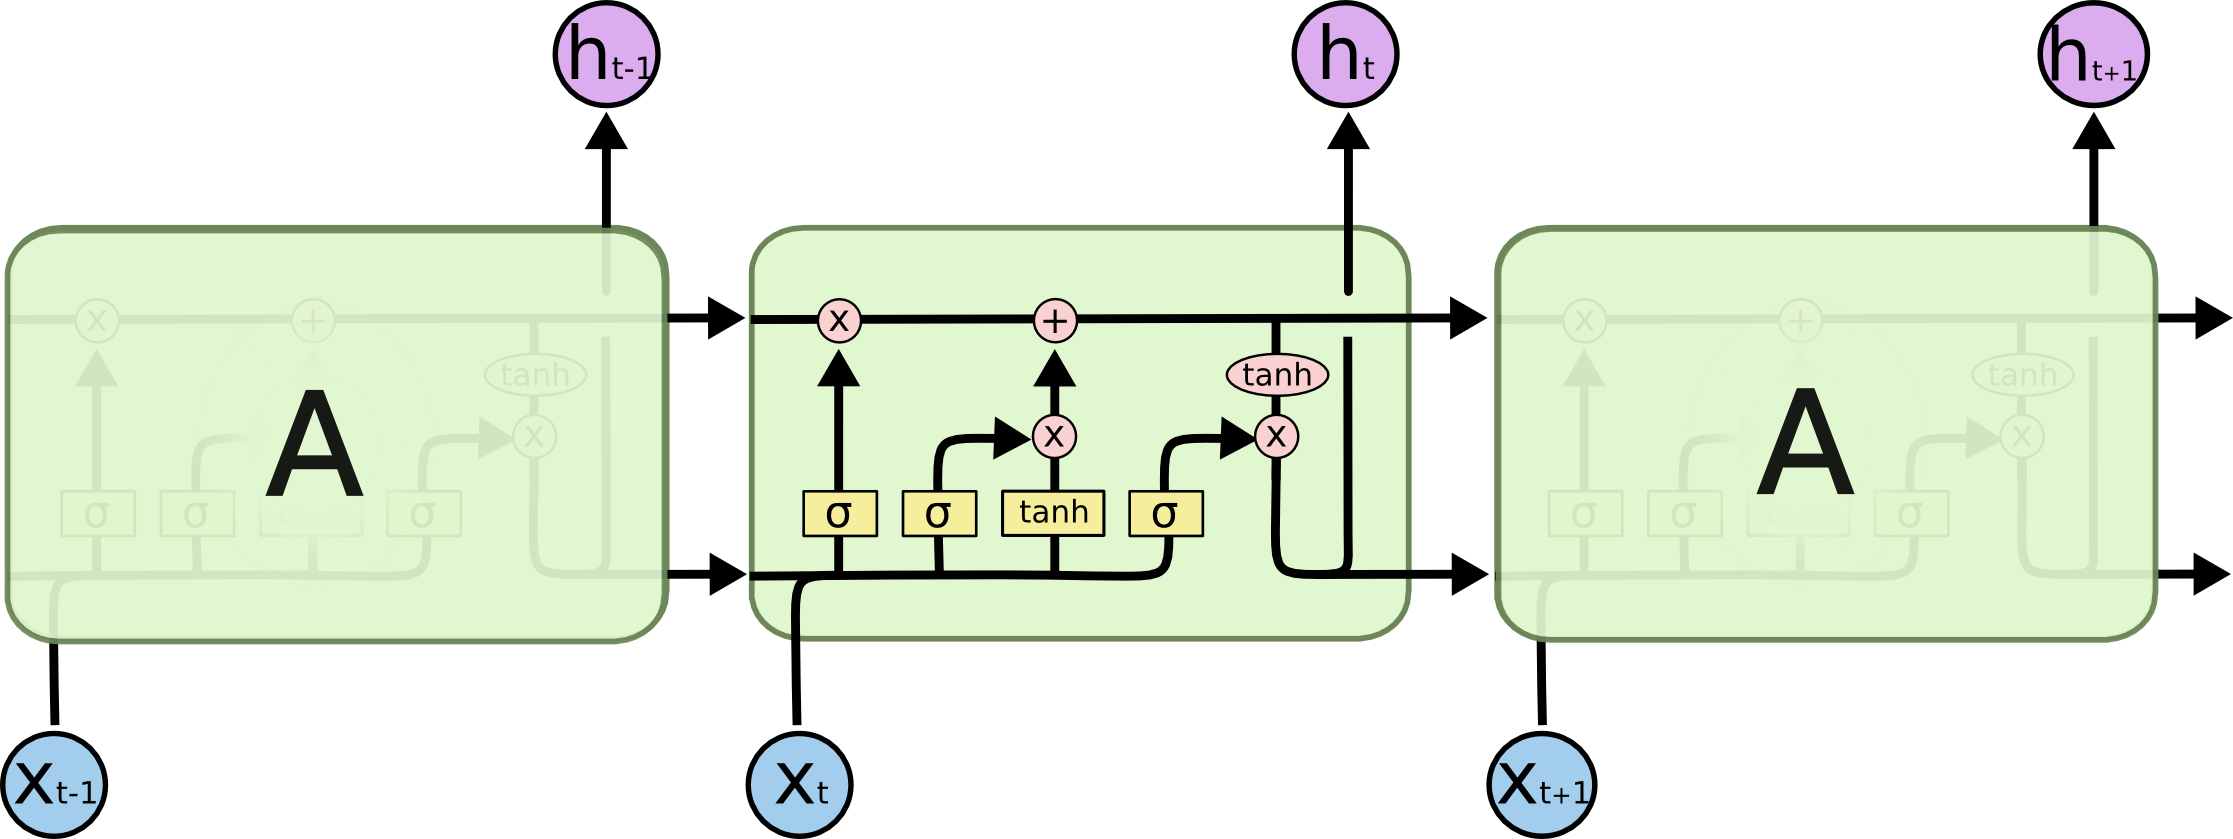
\includegraphics[width=.48\textwidth]{lstm.png}
  \label{fig:lstm_chain}
\end{figure}

A deep LSTM then treats the sequence \(h_t\) as input to another LSTM chain, producing yet another sequence. There can be as many layers as desired. The dimension of \(h_t\) at each layer is a model parameter.

A BiLSTM stands for bidirectional LSTM. It's simply a vanilla LSTM that also considers the sequence in reverse. Then if \(h_t\) is the forward output and \(j_t\) is the backward output, the bidirectional output is
\begin{equation}
  g_t = h_t \oplus j_t
\end{equation}
Note that \(g_t\) has twice as many components as \(h_t\) and \(j_t\) since it's a concatenation of the forward and reverse outputs. The advantage of a BiLSTM over a vanilla LSTM is that a BiLSTM can consider both past and future time steps in producing its output.

The BiLSTM component of my model has 3 layers, with 24, 18, and 12 units going in either direction. It follows that adding a bidirectional component yields 48, 36, and 24 units in total. Each layers has a dropout rate of 0.2, a recurrent dropout rate of 0.4, and L2 kernel and recurrent regularization with \(\lambda = 0.05\). The output activation is \(\tanh\) and the recurrent activation is sigmoid.

The first two layers are sequence-to-sequence, but the final layer is sequence-to-vector. I take only its final output of 24 units and pass it through a fully connected layer with 9 outputs and softmax activation. These values are interpreted as the model's confidence in each accent, as shown in \cref{fig:proba}.
\begin{figure}[h]
  \centering
  \caption{Example Accent Scores}
  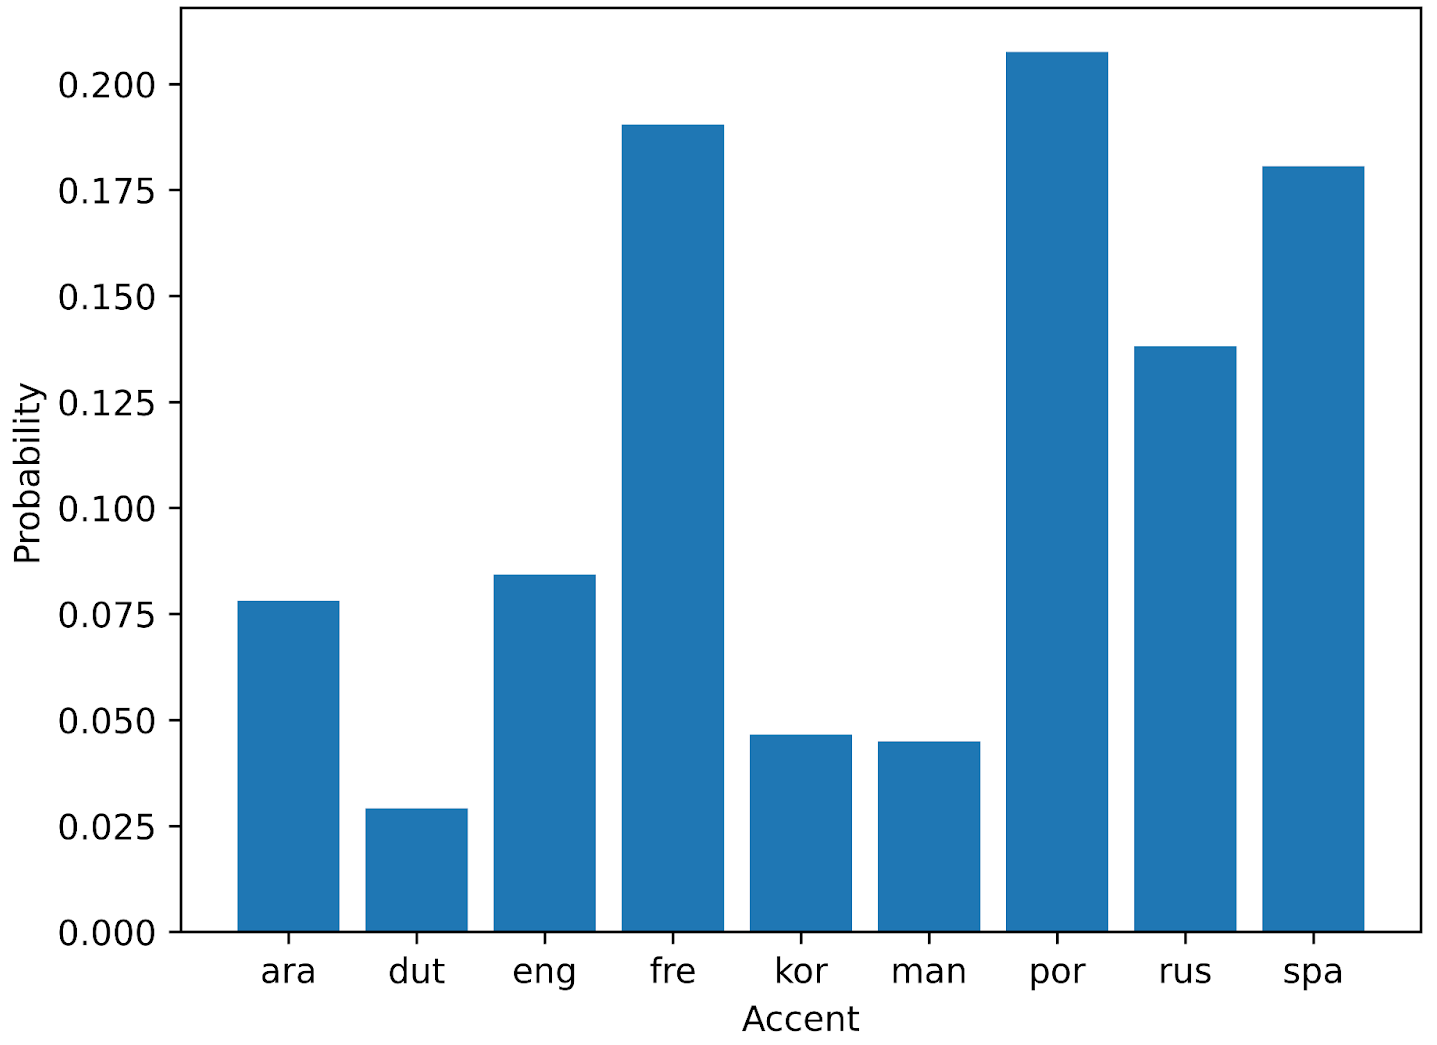
\includegraphics[width=.48\textwidth]{proba.png}
  \label{fig:proba}
\end{figure}

The BiLSTM is capable of learning directly from the mel spectrograms without the CNN component. As such, I use it as a baseline model to be compared with the CNN-BiLSTM.

\section{The CNN} \label{sec:cnn}

Since spectrograms are visual in nature, it makes sense that a convolutional network may learn useful features/representations of the data that can be leveraged in the recurrent phase. In particular, the feature maps preserve the general shape of the time steps and can be interpreted as a sequence in the BiLSTM.

My CNN consists of 4 repeating units of 2-D convolution, max pooling, and dropout layers. The convolution layers are summarized in \cref{tab:conv}.
\begin{table}[h]
  \centering
  \caption{Summary of Convolution layers}
  \begin{tabular}{c|c}
    Filters & Kernel Size    \\
    \hline
    16      & \(5 \times 5\) \\
    32      & \(4 \times 4\) \\
    32      & \(3 \times 3\) \\
    16      & \(3 \times 3\)
  \end{tabular}
  \label{tab:conv}
\end{table}
The convolution kernels are L2 regularized with \(\lambda = 0.05\) and use SAME padding. The activation function is SELU and the kernels are initialized with LeCun normal initialization to take advantage of internal normalization.

Each convolution except the last one is followed by max pooling with pool size of \(2 \times 2\). Finally, a dropout rate of 0.3 is applied at the end of each unit. After 3 layers of max pooling, the \(98 \times 128\) spectrogram is condensed into a shape of \(12 \times 16\). Thus, the final output \(O\) has shape \(12 \times 16 \times 16\), which cannot be passed to the BiLSTM without collapsing the 16 feature maps.

I attempted 2 strategies. The first is to use a global depth (average or max) pool. This produces a BiLSTM input \(I\) of shape \(12 \times 16\) given by
\begin{equation}
  I[t, m] = F(O[t, m, 0], \dotsc, O[t, m, 16 - 1])
\end{equation}
where \(F\) returns either the mean or max of its arguments depending on the choice of average or max pooling. This operation is summarized in \cref{fig:global_pool}.
\begin{figure}[h]
  \centering
  \caption{Global Depth Pooling}
  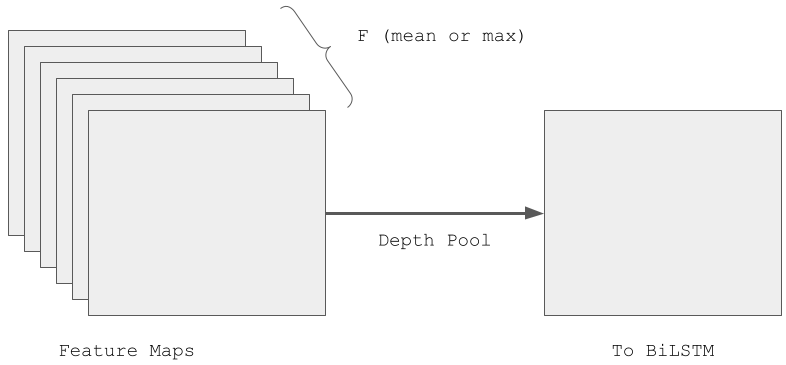
\includegraphics[width=.48\textwidth]{global_pool.png}
  \label{fig:global_pool}
\end{figure}
The major downside to this approach is that this single layer throws out nearly \(94\%\) of the data from the previous layer. I should also note that the mean of 16 feature maps tends to be close to 0. Depth pooling with \(\max\) also tends to produce a relatively constant result, which isn't very useful.

The second strategy (and the one that I implement), is to perform temporal flattening in the sense that I flatten the last 2 dimensions to convert from \(12 \times 16 \times 16\) to \(12 \times 256\) as shown in \cref{fig:temp_flatten}.
\begin{figure}[h]
  \centering
  \caption{Temporal Flattening}
  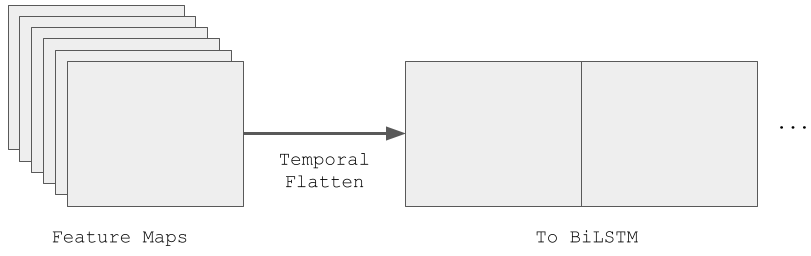
\includegraphics[width=.48\textwidth]{temp_flatten.png}
  \label{fig:temp_flatten}
\end{figure}
This effectively concatenates the mel coefficient axis from all 16 feature maps so that no information is lost going from the CNN to the BiLSTM. Mathematically, this operation is given by
\begin{equation}
  I[t, 16m + c] = O[t, m, c]
\end{equation}
Of course, the downside is that the BiLSTM must now consider many more features in its first layer.

\section{Results} \label{sec:results}

The training process for both the BiLSTM and CNN-BiLSTM were the same. I used a batch size of 32 and 30 epochs. Each model was compiled with an Adam optimizer (initial learning rate of \(0.001\)) and categorical cross entropy loss given by
\begin{equation}
  L(y, p) = -\sum_{i = 0}^{9 - 1} y[i] \cdot \log(p[i])
\end{equation}
where \(y\) is the one-hot encoding of the true label and \(p\) is the softmax output of the model.

To make predictions for a long audio recording, I split it up into \(n\) frames as described in \cref{sec:preprocessing} and apply the model to the spectrogram for each frame. Then, I take the scores for each frame and perform a soft vote to get an aggregate score \(q\) for the entire recording. If \(p_k\) is the softmax output of the \(k^{th}\) frame (0-indexed), then
\begin{equation}
  q = \frac{1}{n} \sum_{k = 0}^{n - 1} p_k
\end{equation}
Then \(q\) may be interpreted as a probability score for each accent.

The curves for training and validation loss of the BiLSTM and CNN-BiLSTM are displayed in \cref{fig:bilstm_loss} and \cref{fig:cnn_bilstm_loss} respectively.
\begin{figure}[H]
  \centering
  \caption{BiLSTM Loss over Training}
  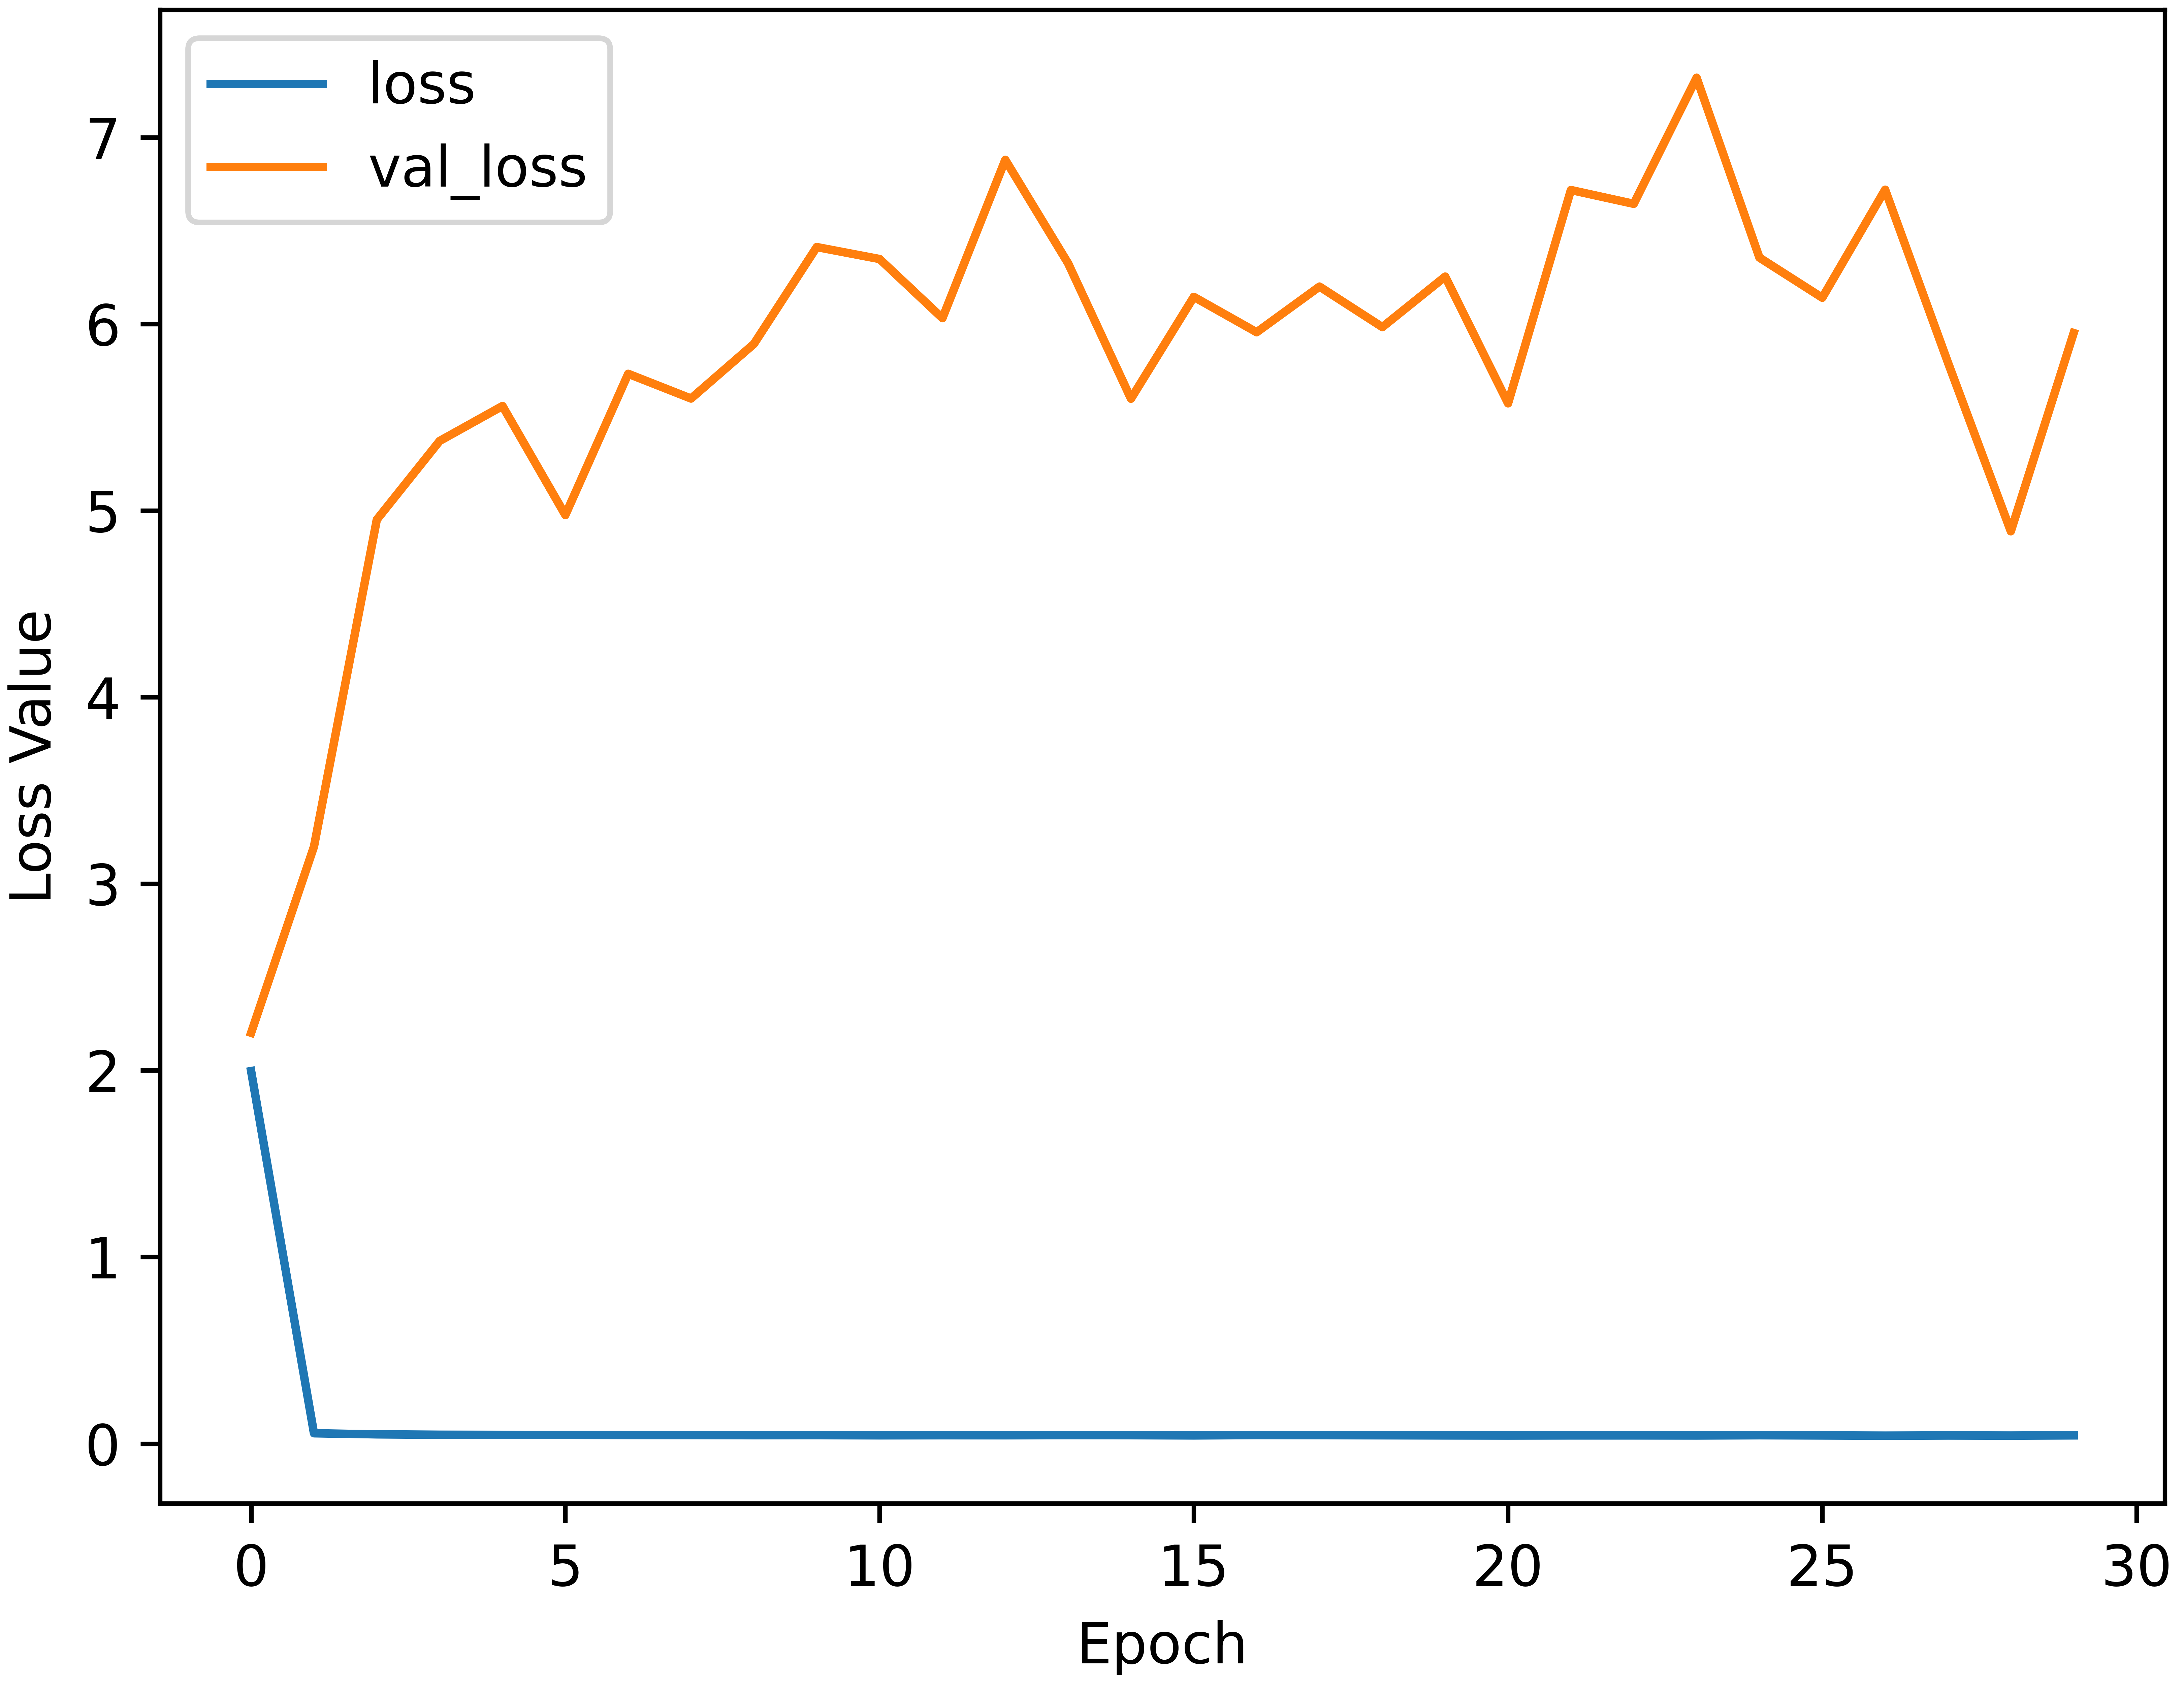
\includegraphics[width=.48\textwidth]{bilstm_loss.png}
  \label{fig:bilstm_loss}
\end{figure}
\begin{figure}[H]
  \centering
  \caption{CNN-BiLSTM Loss over Training}
  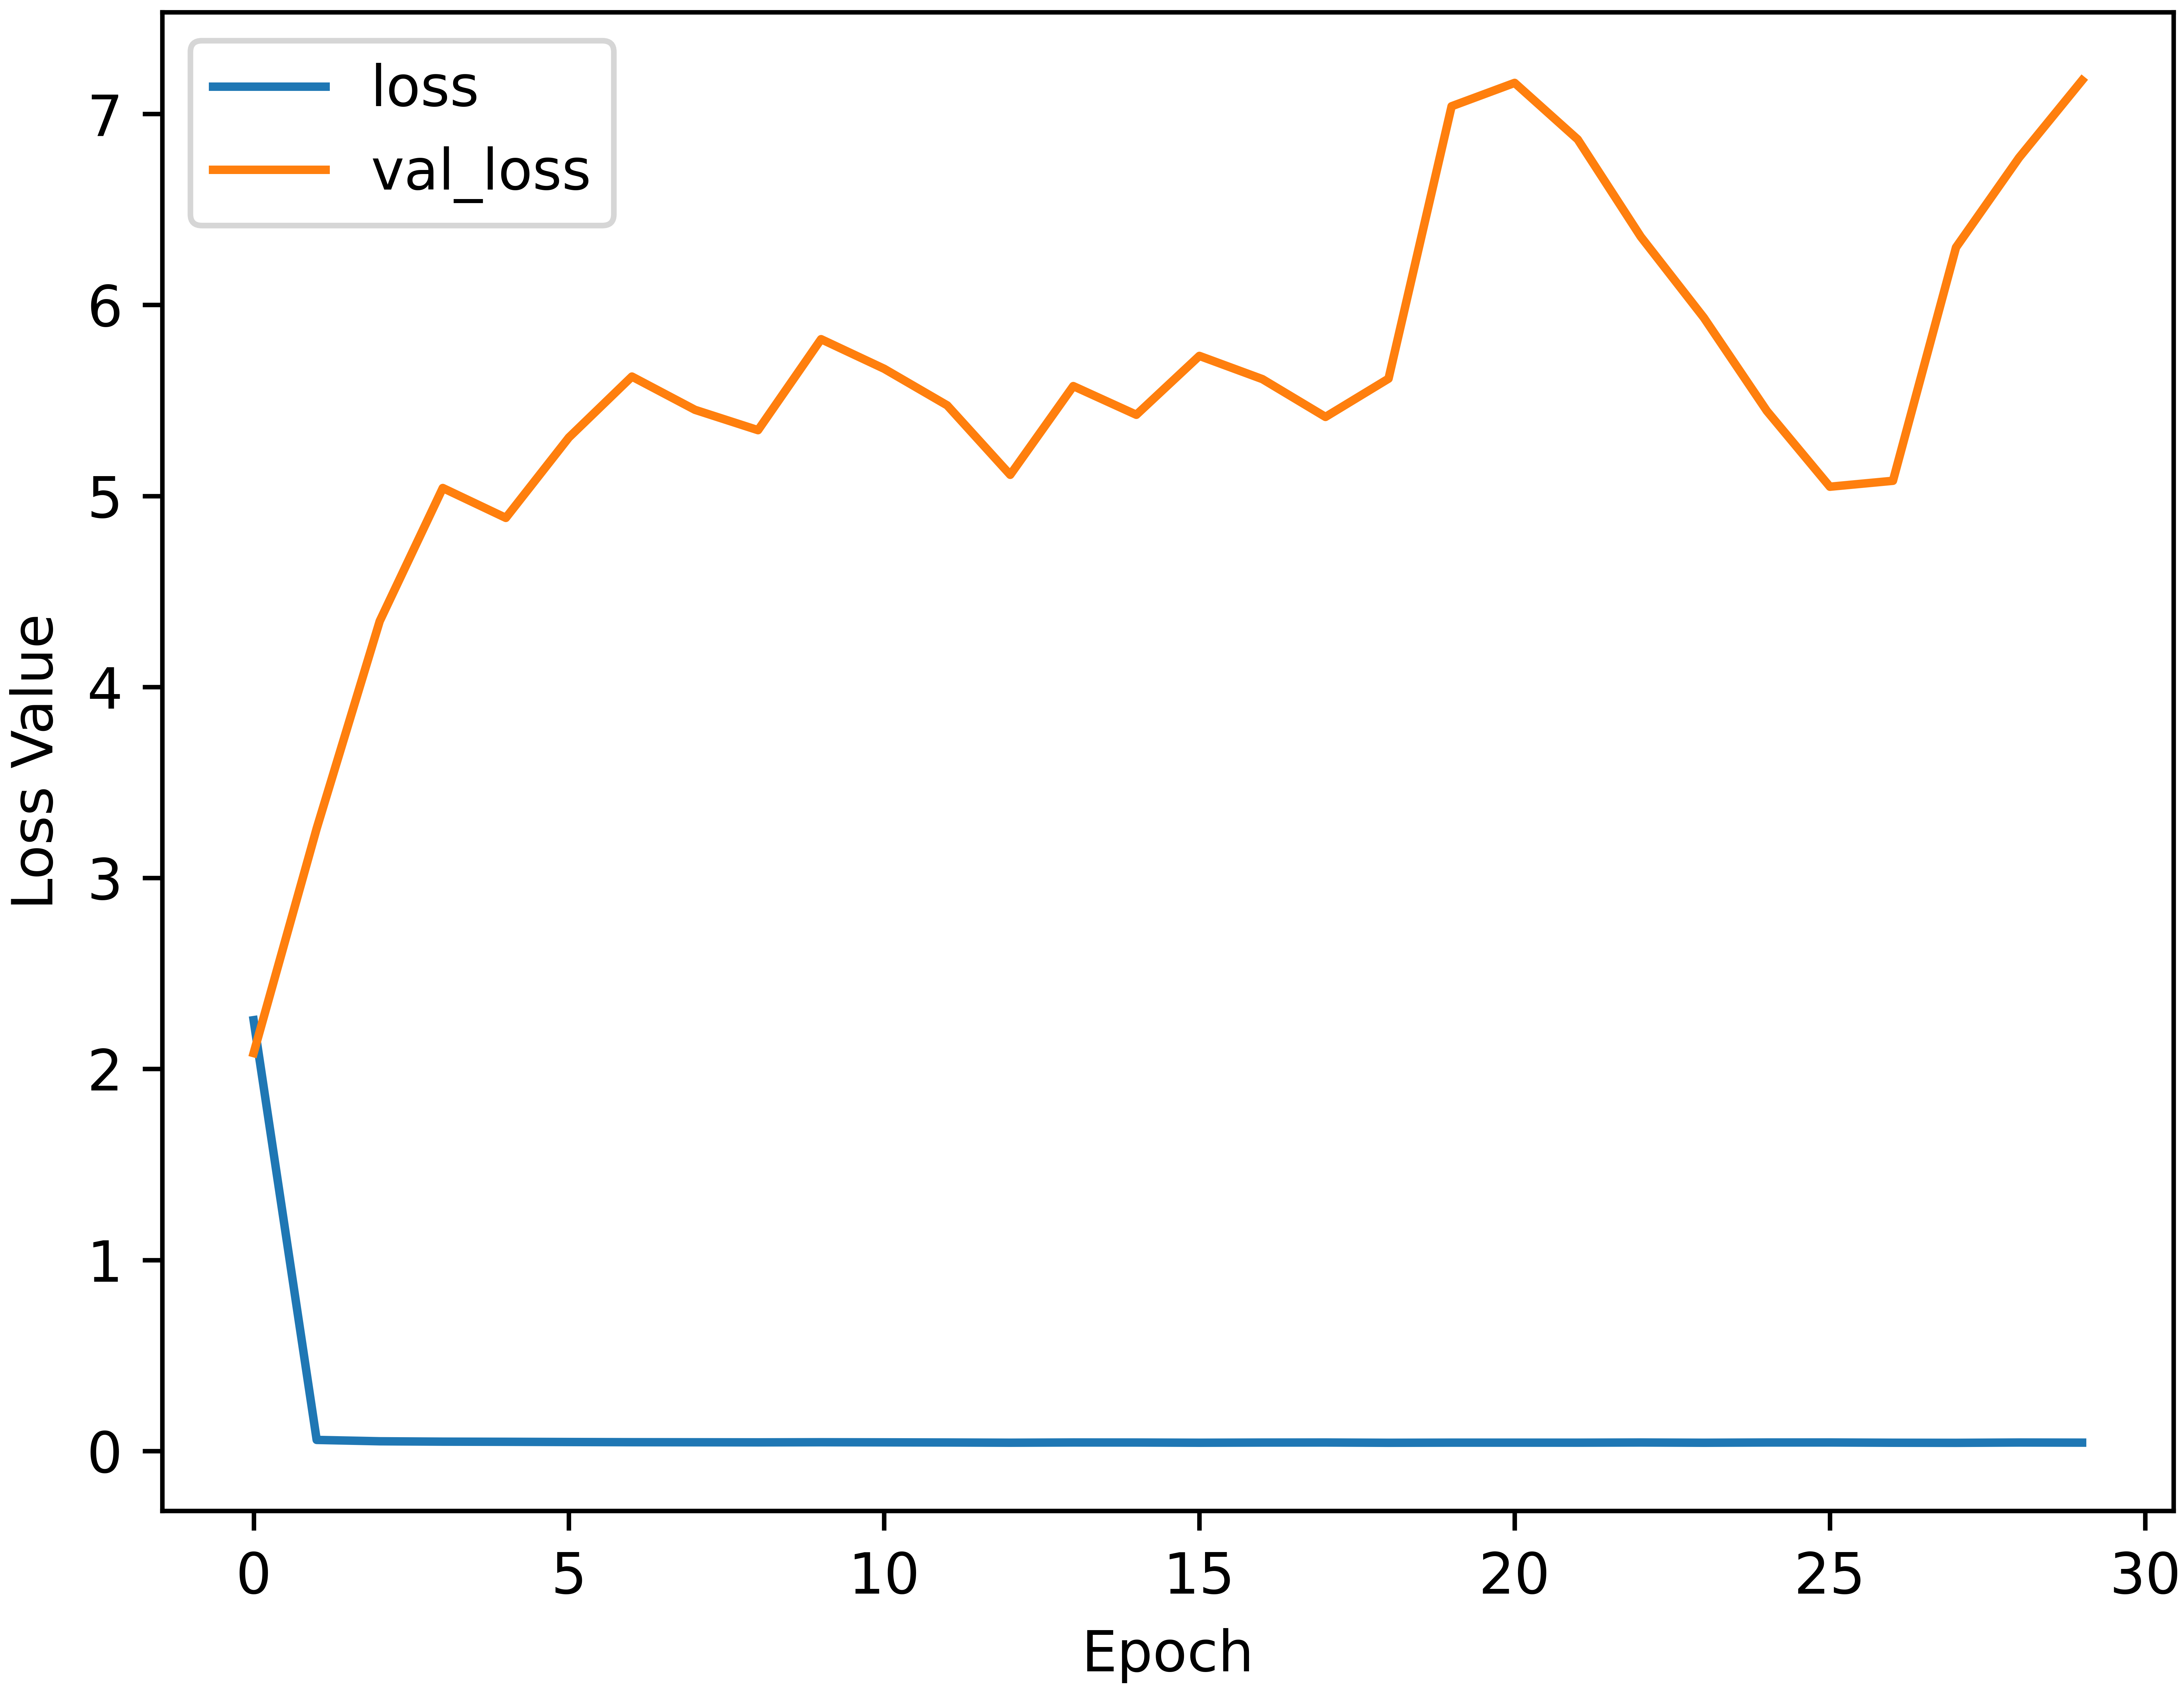
\includegraphics[width=.48\textwidth]{cnn_bilstm_loss.png}
  \label{fig:cnn_bilstm_loss}
\end{figure}

It's apparent that the training process is not stable. Despite experimenting with many model parameters and layers, I always seemed to either underfit or overfit the data. In this case, the model is exhibiting an overfit despite high dropout rates and regularization.

The global depth pooling approach (somewhat unsurprisingly) yielded a more stable training curve, but the results were no better. Average loss on the test set did not dip below \(2.00\) in either of the models, regardless of whether global depth pooling or temporal flattening was used.

Test set results for the best model are summarized in \cref{tab:test_results} where \(S\)-score was defined in \cref{sec:related_work} as how many times more accurate the model is relative to random guessing.
\begin{table}[h]
  \centering
  \caption{Test Results of Best Model}
  \begin{tabular}{c|c|c|c}
    Model      & Loss  & Accuracy & \(S\)-score \\
    \hline
    BiLSTM     & 2.202 & 0.131    & 1.179       \\
    CNN-BiLSTM & 2.083 & 0.134    & 1.206
  \end{tabular}
  \label{tab:test_results}
\end{table}
The results indicate that the CNN did not significantly improve the baseline performance of the BiLSTM. Here, I have defined the ``best'' model as the model with lowest validation loss over the 30 epochs.

To see where the model is lacking, I generated confusion matrices for the best model predicting accents on whole audio recordings. As described previously, I used soft voting to aggregate the frame scores. After standardizing the rows of the confusion matrix, I created heatmaps, which are displayed in \cref{fig:bilstm_heat} and \cref{fig:cnn_bilstm_heat}.
\begin{figure}[H]
  \centering
  \caption{BiLSTM Confusion Matrix}
  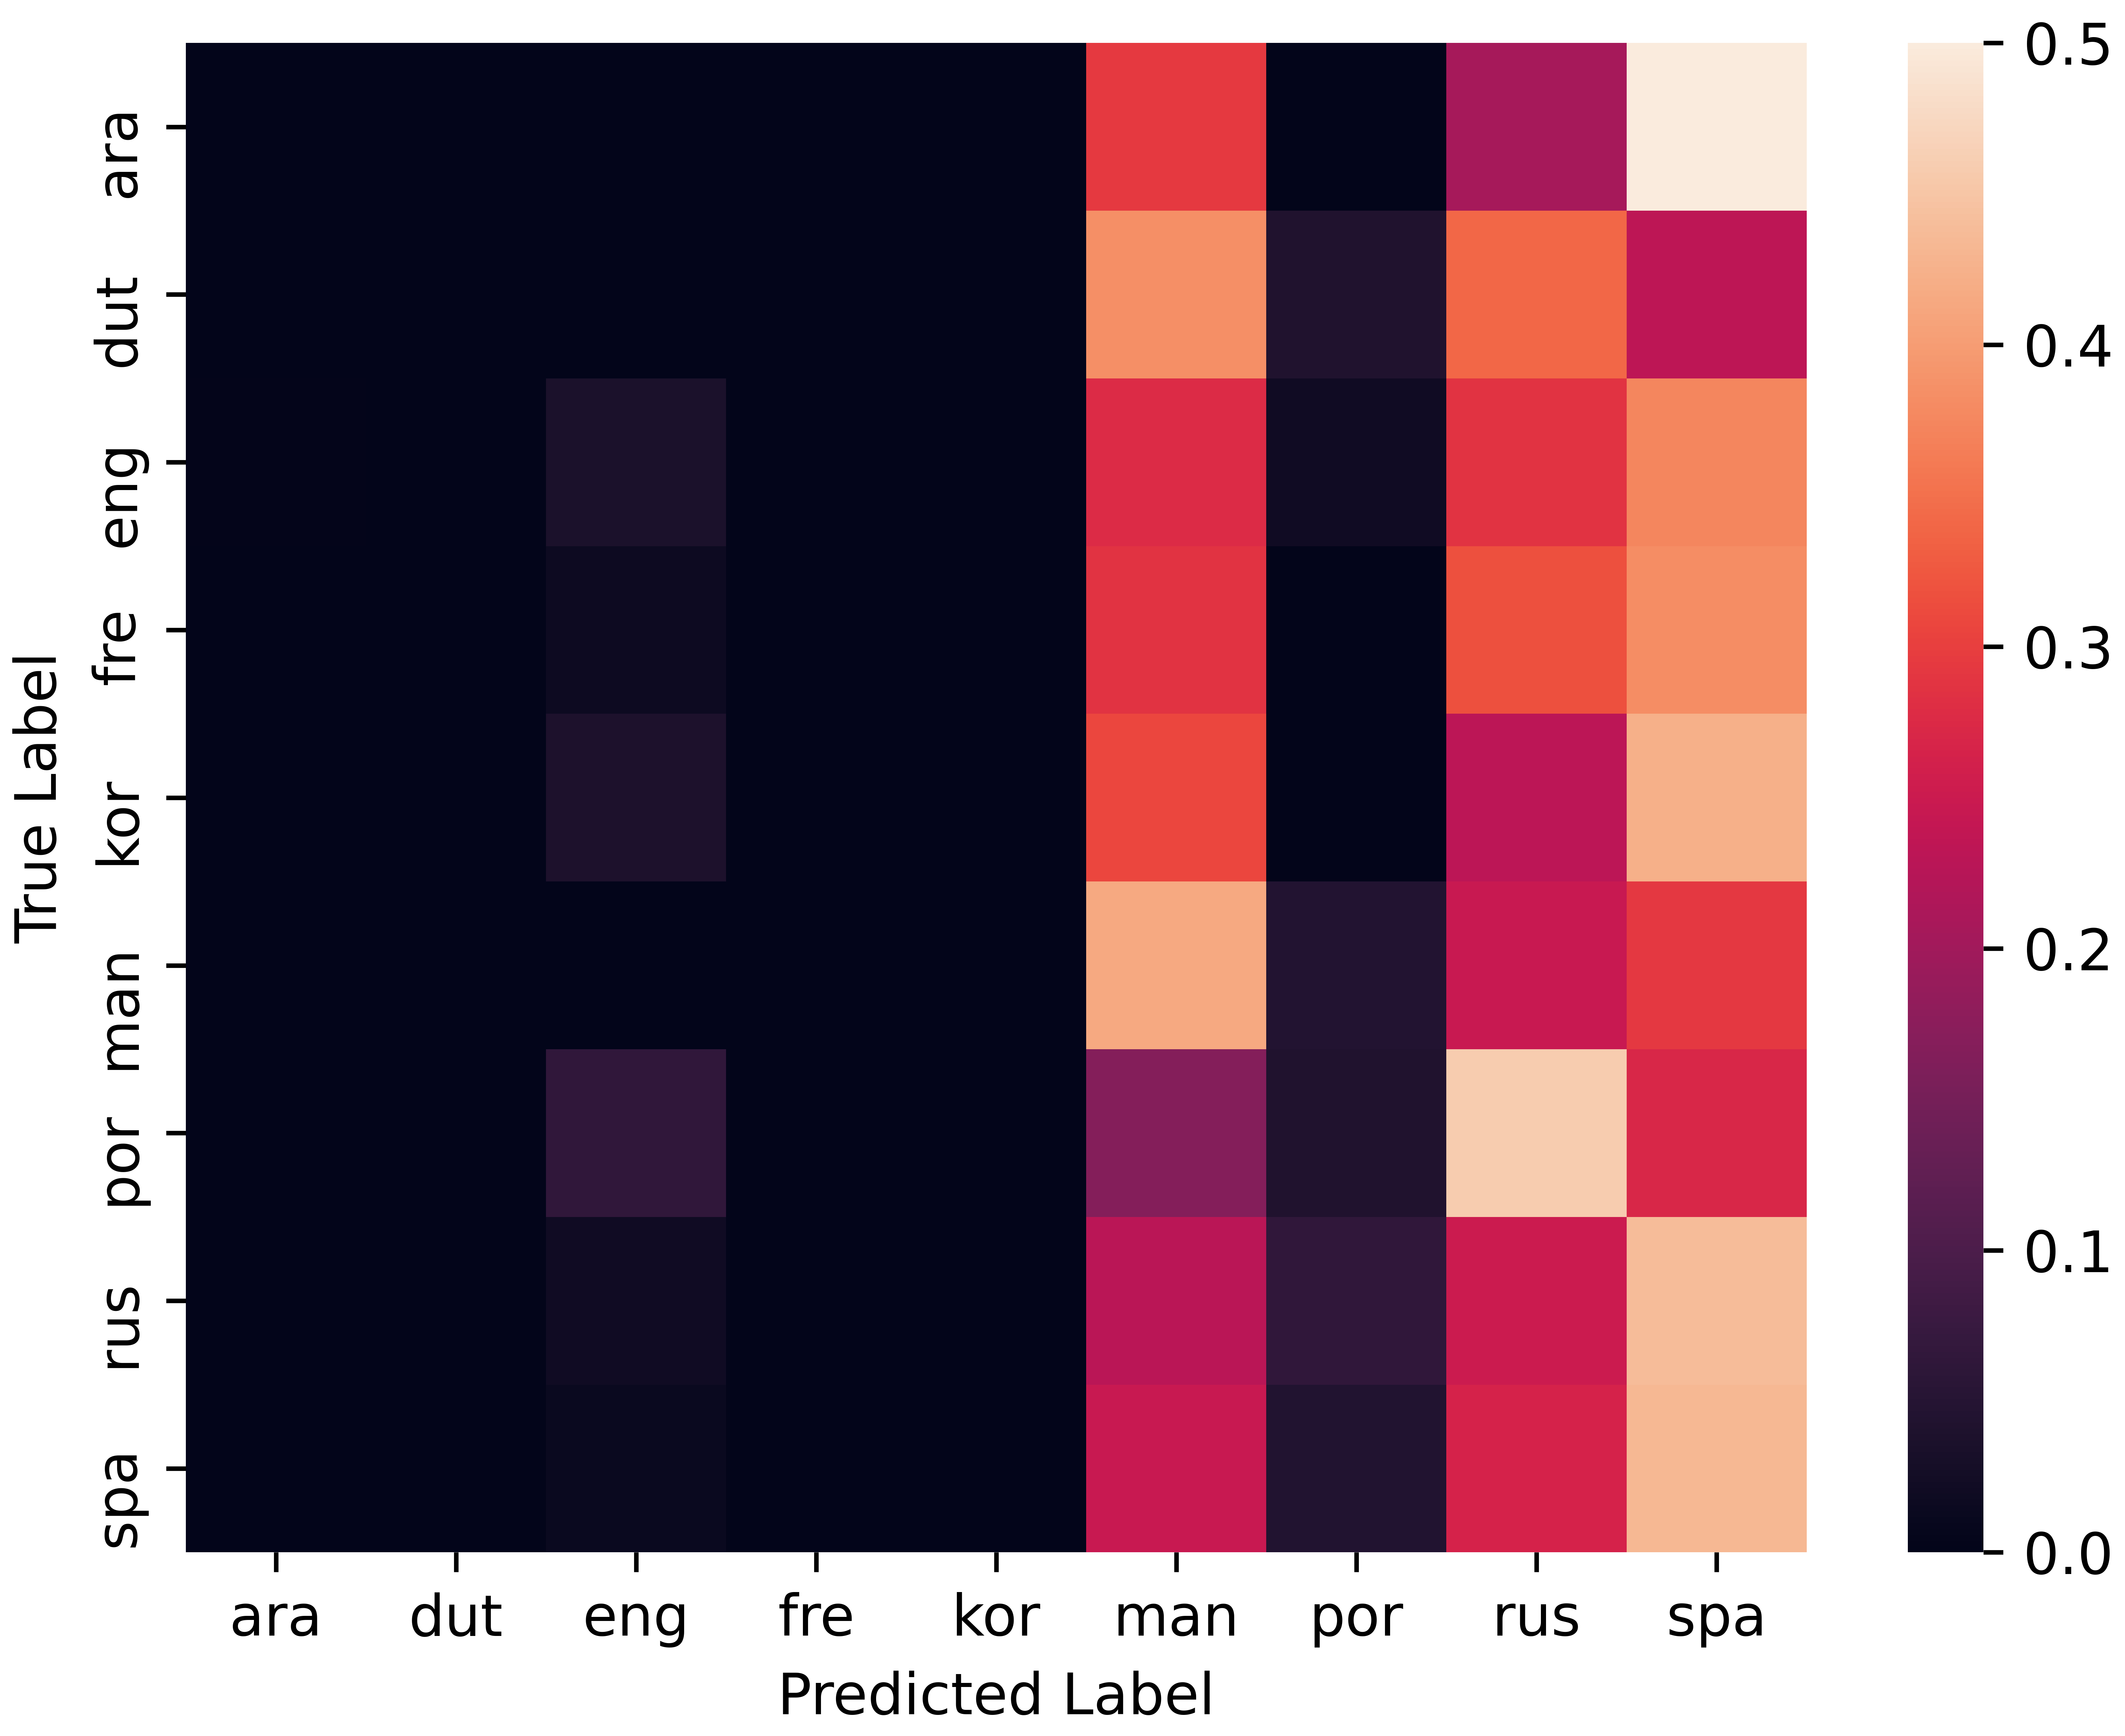
\includegraphics[width=.48\textwidth]{bilstm_heat.png}
  \label{fig:bilstm_heat}
\end{figure}
\begin{figure}[H]
  \centering
  \caption{CNN-BiLSTM Confusion Matrix}
  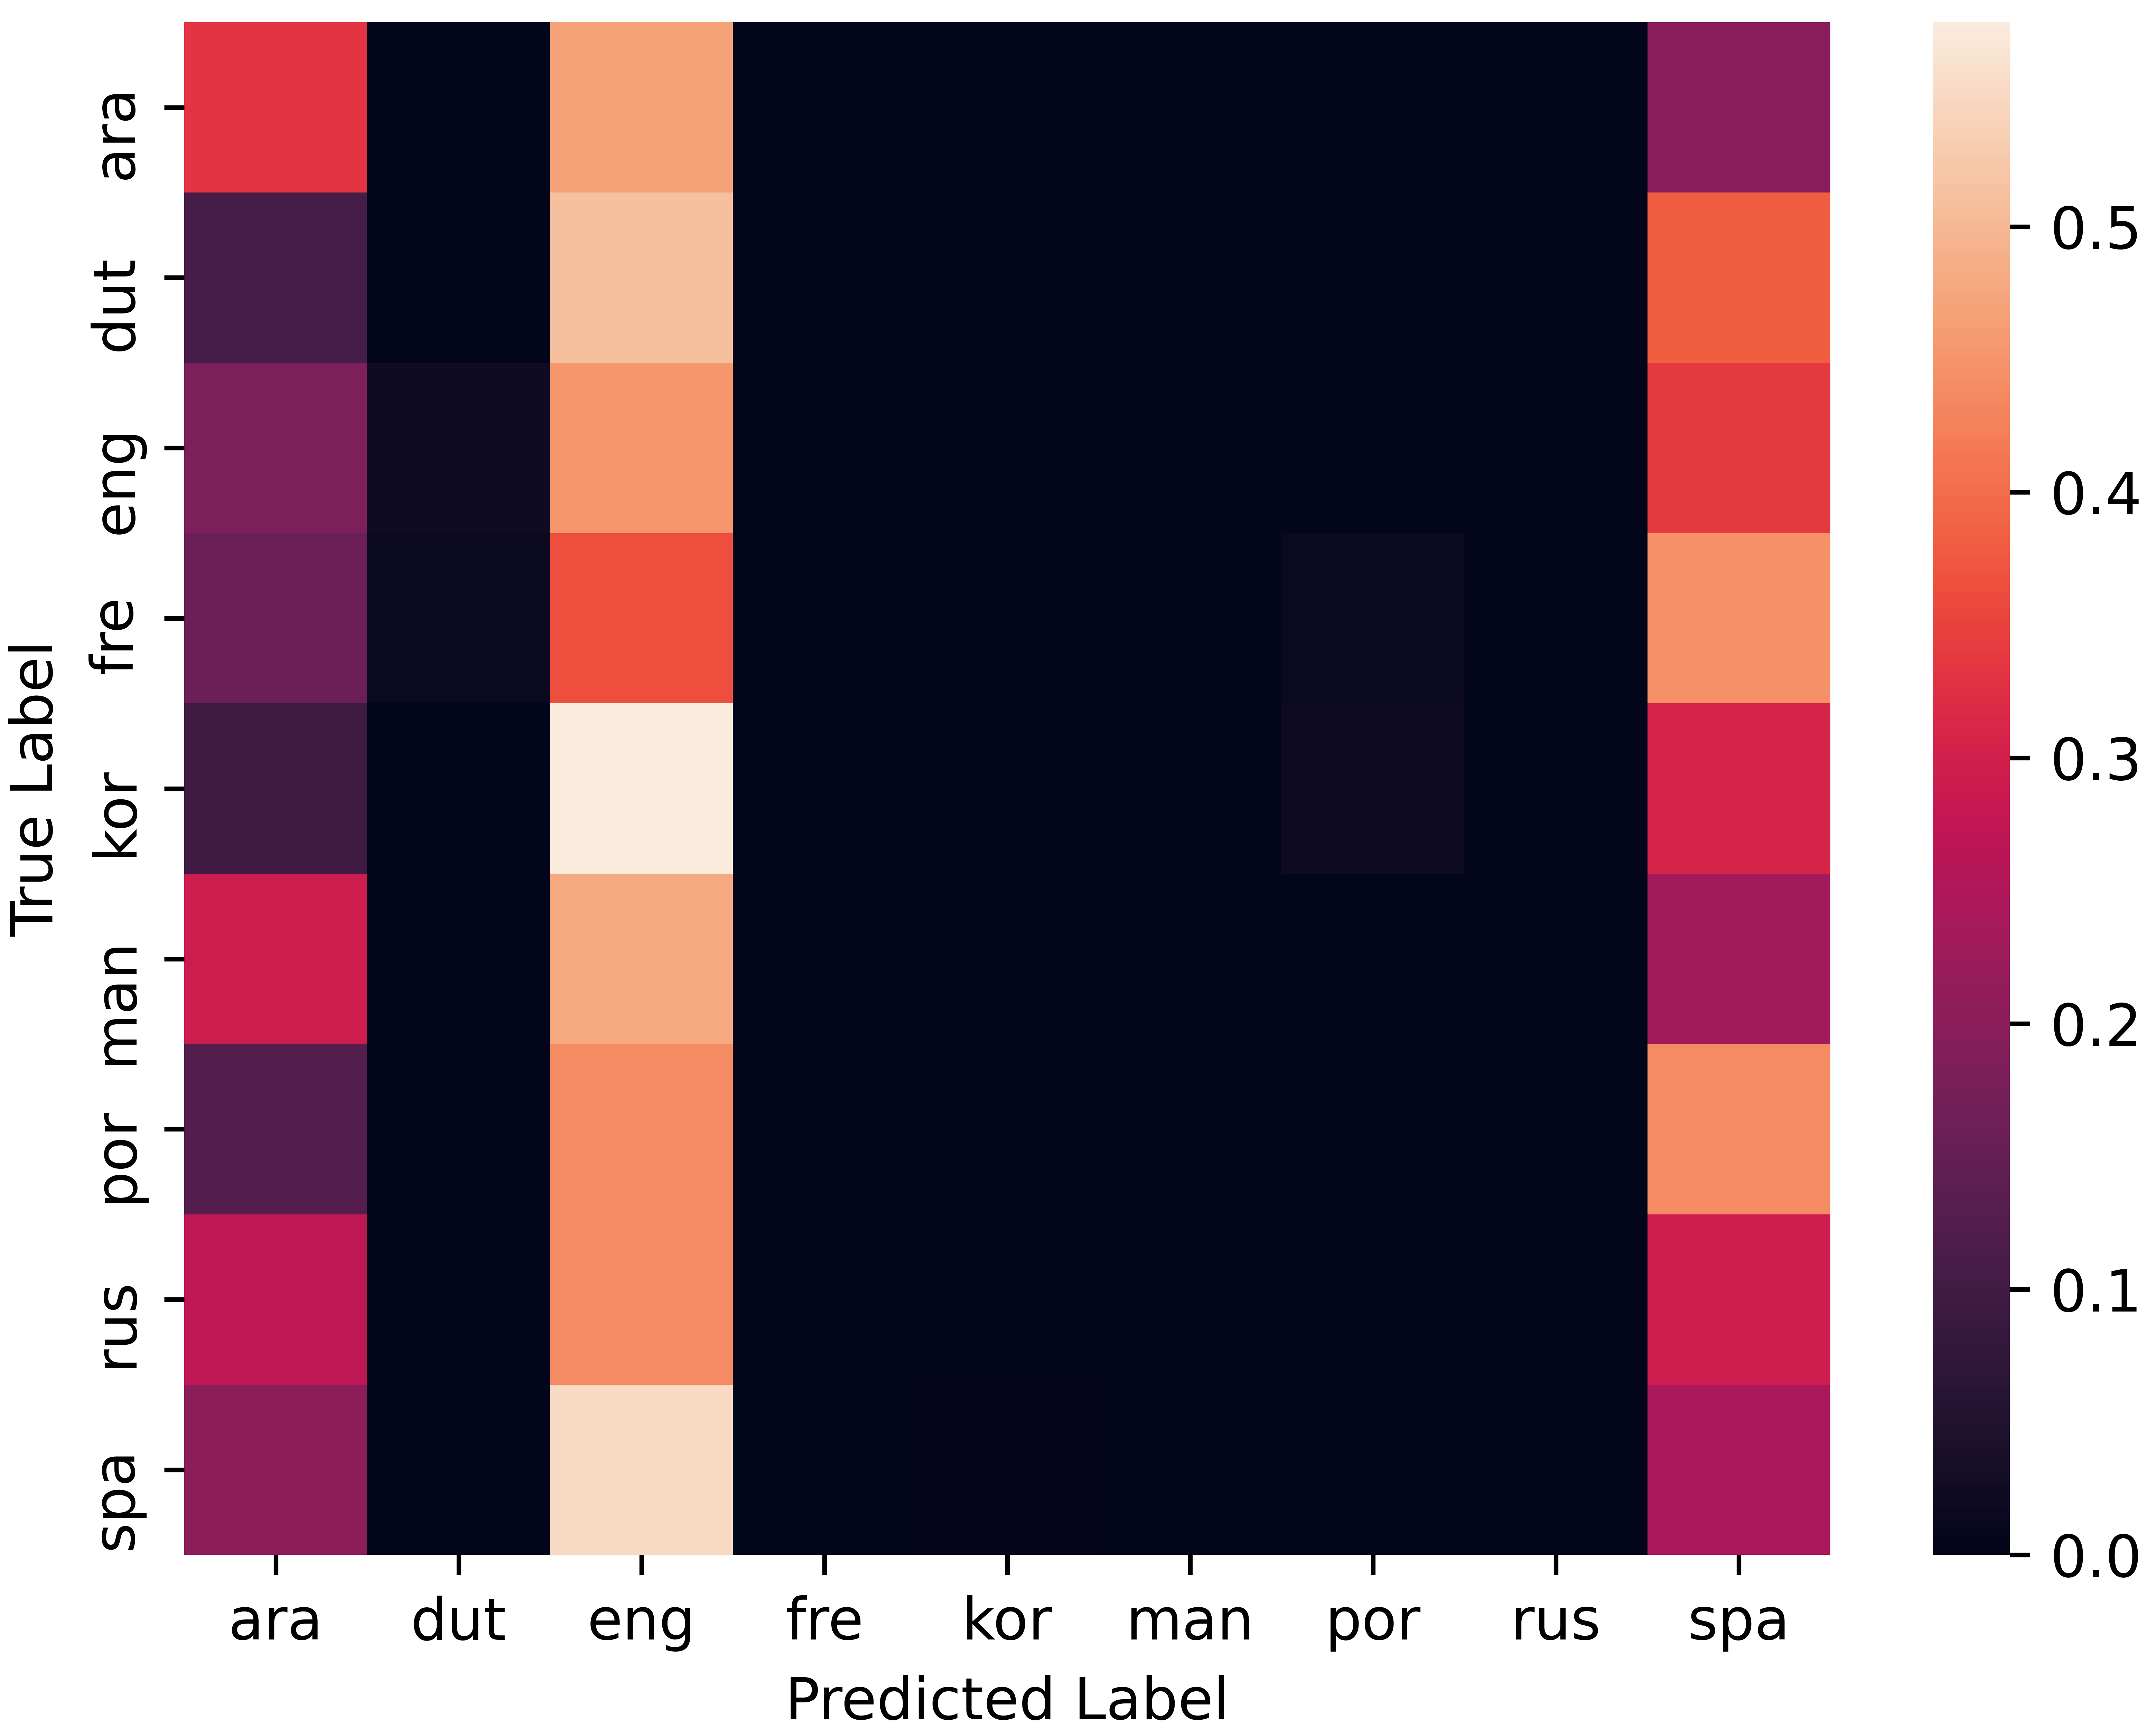
\includegraphics[width=.48\textwidth]{cnn_bilstm_heat.png}
  \label{fig:cnn_bilstm_heat}
\end{figure}

It appears that both models simply avoid predicting a certain subset of the accents. This may indicate that I need to turn down the weight of L2 regression. Other plausible explanations for this phenomena are, as of this writing, unknown to me.

\section{Ethics} \label{sec:ethics}

As with any system that classifies humans, we must take certain precautions in deploying our models and interpreting their results.

One of the most prominent dangers in using ML to label humans is that we can seriously aggravate systemic bias. An accent classifier can be used to predict someone's ethnic background. From my results and that of many others, it’s clear that such a system is not at all reliable. The predictions should not be used to make decisions that will impact people's lives.

Another concern is that most classification models have a finite number of possible labels. In my case, each recording was one of 9 possible accents. This does not reflect the reality that there are hundreds of English accents and many more regional variations. Even if the model was able to perfectly distinguish between the 9 accents, it cannot be applied to individuals with an accent that falls outside of the ones that the model was trained on.

Finally, there is the old adage of ``garbage in, garbage out''. The model could learn the biases and tendencies of the dataset it is trained on. The Speech Accent Archive is relatively gender-balanced and contains accents from a wide variety of geographic locations. However, when training on a new dataset, we should ensure that it does not skew too heavily towards certain demographics more than others. If such biases cannot be avoided in the data, we should at least keep them in mind when interpreting the model's predictions.

\section{Conclusion} \label{sec:conclusion}

One key takeaway I learned from this project is that getting good models for human behavior is hard. The features that differentiate one accent from another are subtle and difficult to describe. While exploring the data, I found that the task of manually determining someone's accent was not as straightforward as I had envisioned.

Despite the performance of the CNN-BiLSTM model leaving much to be desired, I believe there is still much room for improvement. Both convolutional and recurrent networks have the potential to achieve much greater success when it comes to accent classification. Better results may be possible by augmenting the dataset and using a more robust noise removal algorithm. Given greater amounts of data, I believe the models may also benefit from the incorporation of visual attention as surveyed in \citet{attention}.

\bibliographystyle{acl_natbib}
\bibliography{emnlp2020}

\appendix

\section{Supplemental Material}
\label{sec:supplemental}

The dataset and source code to reproduce these results can be found on my Github page at \citet{github}, which is licensed under the permissive MIT License. The repository also includes the tex files and images that produced this paper.

\end{document}
